\documentclass[11pt]{report}

\usepackage{epsf,amsmath,amsfonts}
\usepackage{graphicx}
\usepackage{color}
\usepackage{natbib}

\setlength{\textwidth}{6.5in}
\setlength{\oddsidemargin}{0in}
\setlength{\evensidemargin}{0in}
\setlength{\textheight}{8.5in}
\setlength{\topmargin}{0in}

\begin{document}

\title{
Sub-Ice Shelf Ocean Test
}
\author{MPAS Development Team}

\maketitle
\tableofcontents

%-----------------------------------------------------------------------

\chapter{Summary}

Here we propose a set of tests to answer the following questions:
\begin{enumerate}
\item How thin can MPAs-Ocean layers be compressed below land ice?
\item How steep can the edge of the floating ice shelf be?
\end{enumerate}
The domains are designed to be the simplest possible configurations to test the vertical coordinate, but realistic enough that it provides guidance for global simulations using full bathymetry, forcing, and realistic ice shelves.    The land ice will be imposed with a surface pressure, and MPAS-Ocean will run in 'z-star' mode, where layers contract in proportion to the displaced surface, like an upside-down sigma coordinate.  We hope to demonstrate the extent to which 'z-star' may be used under ice shelves.  the next step would be to make upper cells inactive if z-star does not work.  This is similar to z-level bathymetry but at the top, and is what Xylar implemented in POP.  Likely problems with the z-star formulations for large depressions and slopes are: numerical instabilities in thin layers; tight timestep constraints due to vertical CFL; and velocity errors due to steeply tilted layers.

%-----------------------------------------------------------------------

\chapter{Test Set-up}

The test domain is designed to mimic the geometry of the Pine Island Glacier, which has a steeply sloped ice shelf bottom of 500 m over 30 km (Figure \ref{figure:pig observations}, \citet{Jenkins_ea10ngeo}).  Parameters are listed in Table \ref{table:ideal test parameters}.  The ocean will be run in stand-alone mode, without a land ice model or coupler.  There will be no fluxes from the ice shelf, and the ocean will be depressed but a surface pressure due to the weight of the ice shelf.

The ocean will consist of 22 layers that compress proportionally below the ice sheet, so that they are each 50 m thick in the open ocean and 4.5 m thick at the inlet (Figure \ref{figure:ice shelf domain}a).  The inlet thickness, $A$, will be varied from 100m to 1m to test how thin the layers may function properly.  The inlet thickness will be decreased by increasing the surface pressure so that the whole ice sheet is uniformly deeper.  The upper slope at the end of the ice shelf will be controlled by varying $B$ from 0 to 30 km, to test the model's ability to include steep slopes.

The inflow water has a salinity of 34.3 psu, which is more buoyant than the surface water, so it will follow the ice shelf slope upward.  It enters at a constant volume flux of $10 D_x$ m$^2$/s, where $D_x$ is the domain size in the periodic $x$ direction.  This produces an inflow with a speed of 10 cm/s when the inlet is 100 m deep.  The volume flux may need to be reduced when testing thin inlets.  

In addition to the flat-bottom case, bathymetry may be added to show the combination of z-level land cells with compressed z-star layers (Figure \ref{figure:ice shelf domain}b).


\begin{figure}[tbh]
\center
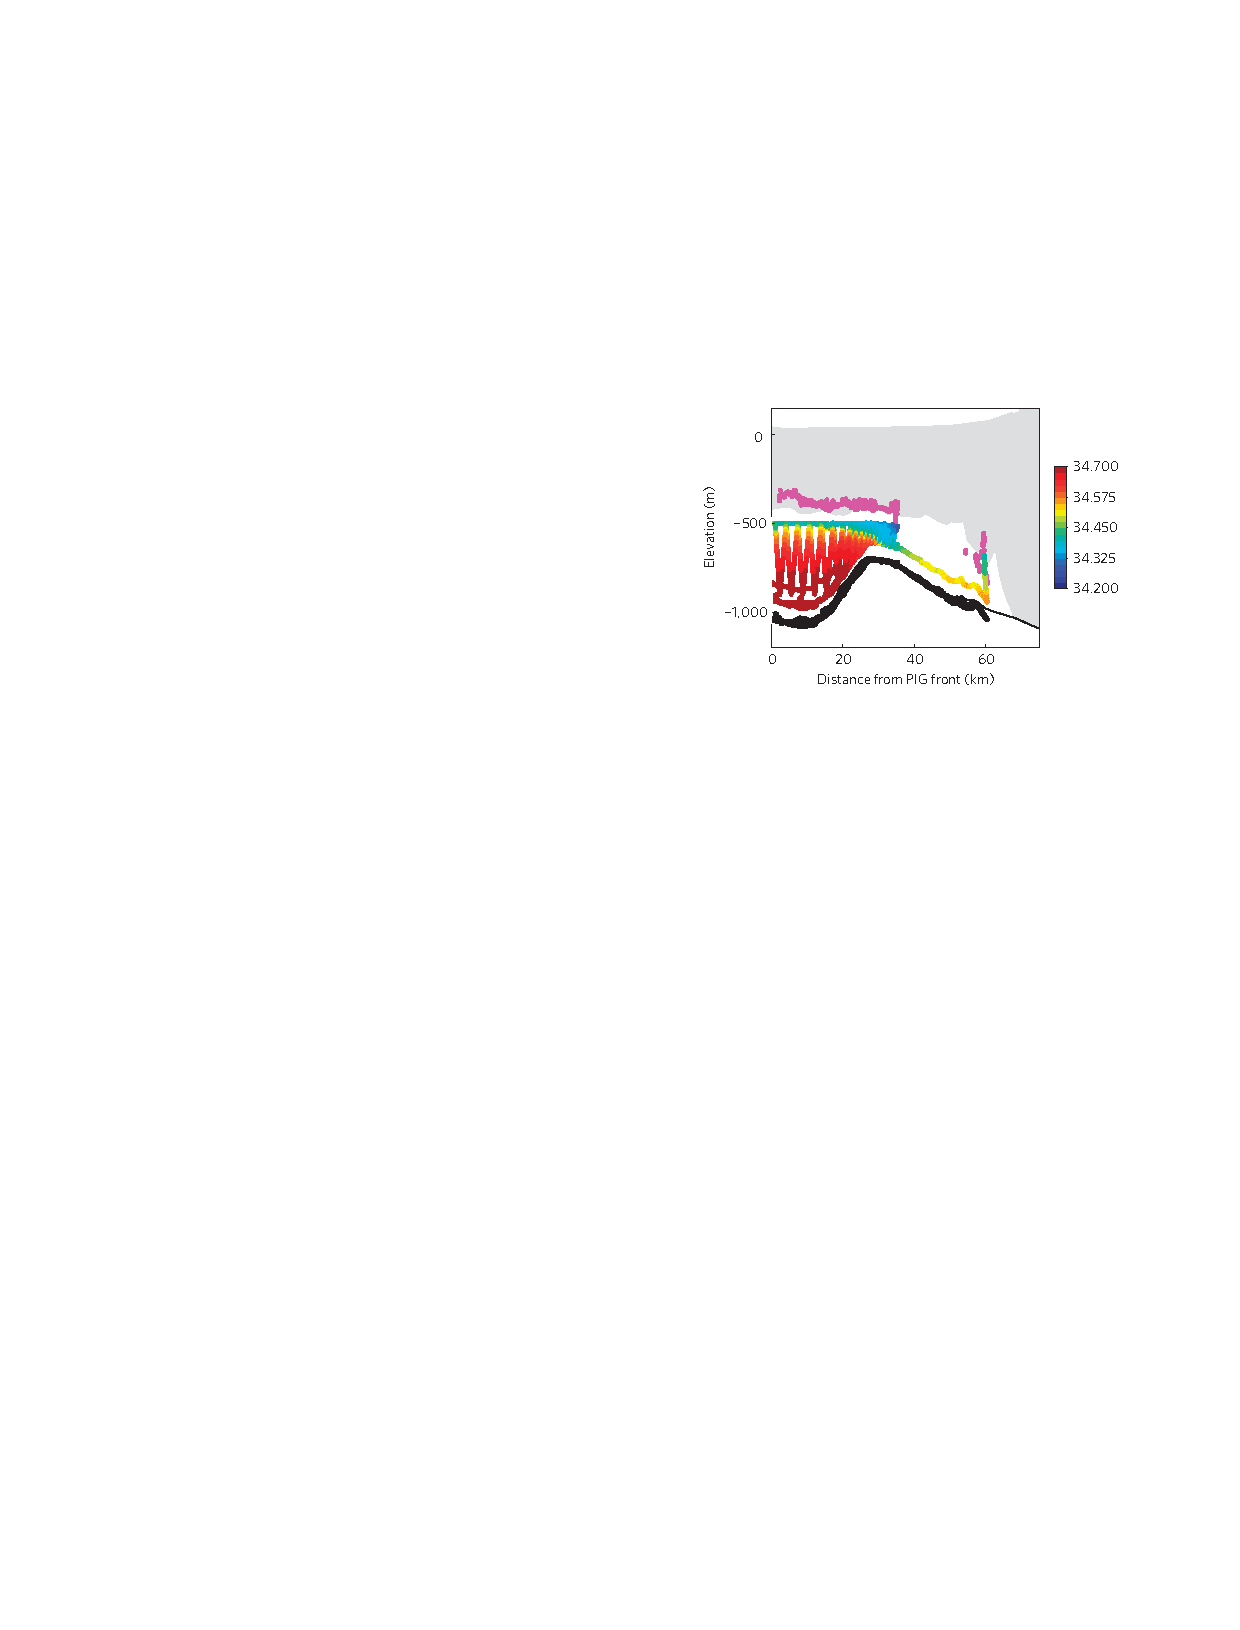
\includegraphics[width=3in]{f/Jenkins_ea10ngeo_fig4b.pdf}
\caption{Observations below the Pine Island Glacier, from \citet{Jenkins_ea10ngeo}.  Ocean salinity and slope of the ice shelf were considered in designing the test domain.}
\label{figure:pig observations}
\end{figure}

\begin{figure}[tbh]
\center
(a)\includegraphics[width=6.5in]{f/sub-ice_shelf_diagram1.pdf}\\
\vspace{.2in}
(b)\includegraphics[width=6.8in]{f/sub-ice_shelf_diagram2c.pdf}
\caption{Domain of the ice shelf test case: (a) standard configuration and (b) addition of z-level topography.  The inlet thickness (A) and width of ice shelf edge (B) are the parameters that will be varied.}
\label{figure:ice shelf domain}
\end{figure}


\begin{table}[tbh] 
\caption{Parameter settings for sub-ice shelf test cases.}
\vspace{0.5cm} \centering 
\begin{tabular}{r|c } 
\hline\hline & case 1 \\
\hline 
domain size $x$ &  2 grid cells, periodic \\
domain size $y$ & 200 km\\
domain size $z$ &  1100 m \\
number layers& 20 \\
layer thickness & 50 m in open ocean \\
grid cell size, km  & 15, 5, 1 \\
time step $\Delta t$, s & 600, 200, 40 \\
$\nu_h$, m$^2/$s & 5e10, 1.8e9, 1.5e7 \\
$\nu_v$, m$^2/$s & rich, bkrd of $1\times10^{-4}$ \\
$\kappa_h$, m$^2/$s & 0 \\
$\kappa_v$, m$^2/$s & rich, bkrd of $1\times10^{-5}$ \\
bottom drag & 0.01 \\
Coriolis, s$^{-1}$ & off \\
run duration& 30 days \\
\hline 
\end{tabular} \label{table:ideal test parameters}
\end{table}

%-----------------------------------------------------------------------

\bibliographystyle{elsarticle-harv}
\bibliography{sub-ice_shelf_ocean_test}

%-----------------------------------------------------------------------

\end{document}
